\documentclass{article}%
\usepackage[T1]{fontenc}%
\usepackage[utf8]{inputenc}%
\usepackage{lmodern}%
\usepackage{textcomp}%
\usepackage{lastpage}%
\usepackage[head=40pt,margin=0.5in,bottom=0.6in]{geometry}%
\usepackage{graphicx}%
%
\title{\textbf{Ellos y Venezuela}}%
\author{CAROLINA JAIMES BRANGER}%
\date{04/03/2019}%
%
\begin{document}%
\normalsize%
\maketitle%
\textbf{URL: }%
http://www.eluniversal.com/el{-}universal/34442/ellos{-}y{-}venezuela\newline%
%
\textbf{Periodico: }%
EU, %
ID: %
34442, %
Seccion: %
el{-}universal\newline%
%
\textbf{Palabras Claves: }%
NO\_TIENE\newline%
%
\textbf{Derecho: }%
2.1%
, Otros Derechos: %
\newline%
%
\textbf{\textit{La alegría de ayudar es inconmensurable. Y sentirse apoyado en tiempos difíciles es una necesidad. Juego en la computadora “Apalabrados”, con personas de distintos países.}}%
\newline%
\newline%
%
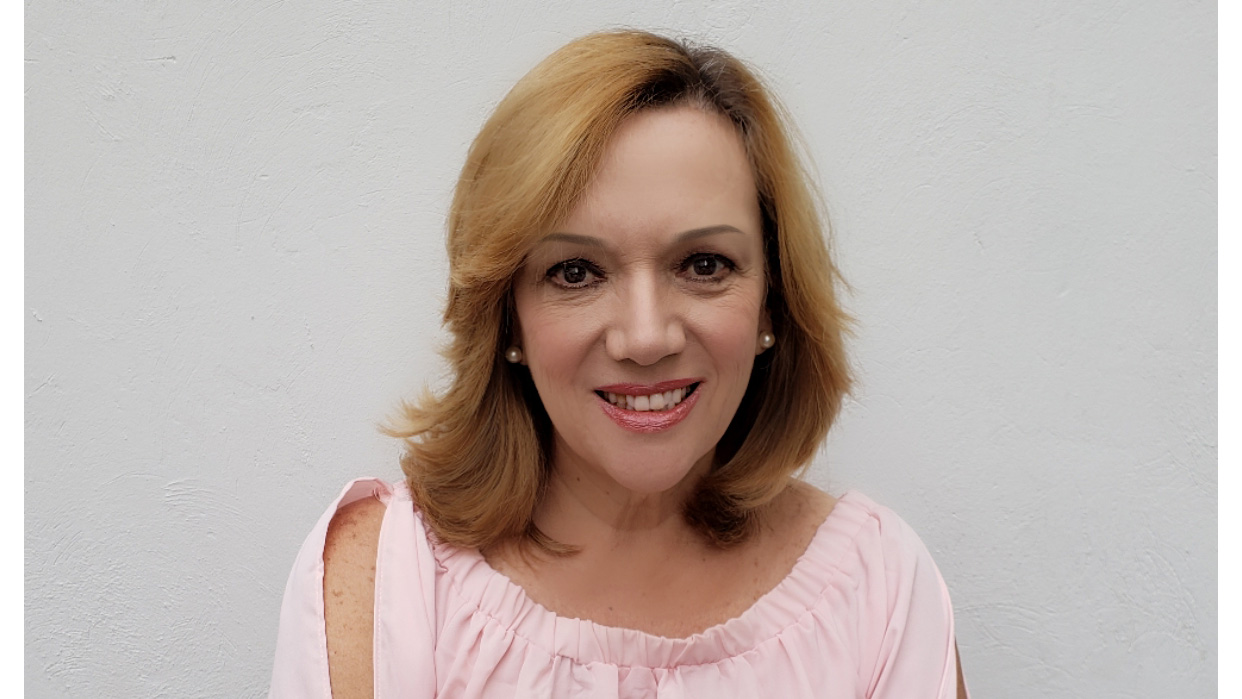
\includegraphics[width=300px]{EU_34442.jpg}%
\newline%
%
Esta tragedia que vivimos –como todo en la vida– ha traído sus cosas buenas. Hoy quiero referirme a quienes no son venezolanos, pero aún así han tomado la bandera de nuestra situación para hacerla visible, apoyar y encontrar ayuda.%
\newline%
%
Por supuesto, en primera línea están los periodistas. A Fernando Del Rincón habrá que hacerle una estatua en alguna plaza pública. Lo mismo a Jaime Bayly. A Andrés Oppenheimer, Mario Vargas Llosa, Plinio Apuleyo Mendoza, mi más sentida gratitud como venezolana. Luego, los políticos: al Senador Marco Rubio y al Secretario General Luis Almagro no tendremos suficientes palabras de agradecimiento ni tiempo para que haya reciprocidad. A la Eurodiputada Beatriz Becerra, quien ha defendido a nuestro país como si se tratara del suyo. A Mark Green de USAID por su perseverancia en que llegue la ayuda humanitaria... Y así como ellos –y pido disculpas por todos los que deberían estar mencionados– miles alrededor del mundo.%
\newline%
%
Pero hay otros apoyos de los que sólo sabemos quienes tenemos contacto con personas no venezolanas, que constante y consistentemente están pendientes de nuestra situación. Todos tenemos cerca a muchos y saben a qué me refiero... Y merecen igualmente nuestro reconocimiento y retribución. Sólo espero que sus países no tengan que pasar por lo que pasa el nuestro.%
\newline%
%
Son personas que están pendientes y presentes. Pienso, por ejemplo, en el señor Carlo Lomonte, un seguidor mío en Twitter, que vive en Italia. Él me escribió una vez porque vio que yo estaba pidiendo un remedio que no se conseguía (para variar). Me contó que él había vivido en Venezuela, a la que agradecía muchas cosas. Que se sentía muy mal por lo que estábamos pasando y quería ayudar. Ya he recibido varios envíos suyos para paliar las necesidades de personas que no conoce, pero que siente como suyas. ¡Ésa es la verdadera generosidad! Y nombro al señor Lomonte, ¡pero hay tantos como él!%
\newline%
%
La alegría de ayudar es inconmensurable. Y sentirse apoyado en tiempos difíciles es una necesidad. Juego en la computadora “Apalabrados”, con personas de distintos países. Todos ellos me contactan con frecuencia para saber cómo estoy y cómo pueden ayudar. Es reconfortante. Frente a la ignominia, dignidad. Frente a la ruindad, nobleza. Frente a la canallada, desprendimiento. ¡Los buenos somos más!%
\newline%
%
@cjaimesb%
\newline%
%
\end{document}